\testfile{pgfplotstest.enlargelimits.tex}
\testsection{Limit computation}
\testsubsection{User specified limits}
{
\pgfplotsset{every axis/.append style={
	scaled ticks=false,enlargelimits=false,
	extra x ticks={-40,40},
	extra y ticks={-37760,24960},
	}}
[scaled ticks = false,enlargelimits=false] in this section
\testsubsubsection{linear plot, unconstraint}
\begin{tikzpicture}
	\begin{axis}
		\addplot file{plotdata/pgfplots.testplot};
	\end{axis}
\end{tikzpicture}

\testsubsubsection{linear plot, limited to $x \in [-20,20]$}
\begin{tikzpicture}
	\begin{axis}[xmin=-20,xmax=20]
		\addplot file{plotdata/pgfplots.testplot};
	\end{axis}
\end{tikzpicture}

\testsubsubsection{linear plot, limited to $y \in [-12000,800]$}
\begin{tikzpicture}
	\begin{axis}[ymin=-12000,ymax=800]
		\addplot file{plotdata/pgfplots.testplot};
	\end{axis}
\end{tikzpicture}

\testsubsubsection{linear plot, limited to $x \in [-20,20]; y \in [-12000,800]$}
\begin{tikzpicture}
	\begin{axis}[xmin=-20,xmax=20,ymin=-12000,ymax=800]
		\addplot file{plotdata/pgfplots.testplot};
	\end{axis}
\end{tikzpicture}

\testsubsubsection{linear plot, limited to empty $x$-range}
\begin{tikzpicture}
	\begin{axis}[xmin=2000,xmax=20000]
		\addplot file{plotdata/pgfplots.testplot};
	\end{axis}
\end{tikzpicture}

\testsubsubsection{linear plot, limited to xmin=18}
\begin{tikzpicture}
	\begin{axis}[xmin=18]
		\addplot file{plotdata/pgfplots.testplot};
	\end{axis}
\end{tikzpicture}

\testsubsubsection{linear plot, limited only in xmax=18}
\begin{tikzpicture}
	\begin{axis}[xmax=18]
		\addplot file{plotdata/pgfplots.testplot};
	\end{axis}
\end{tikzpicture}


\testsubsubsection{linear plot, limited only in ymin=-12000}
\begin{tikzpicture}
	\begin{axis}[ymin=-12000]
		\addplot file{plotdata/pgfplots.testplot};
	\end{axis}
\end{tikzpicture}

\testsubsubsection{linear plot, limited only in ymax=-12000}
\begin{tikzpicture}
	\begin{axis}[ymax=-12000]
		\addplot file{plotdata/pgfplots.testplot};
	\end{axis}
\end{tikzpicture}

\testsubsubsection{linear plot, clip limits=false and xmin = 50}
\begin{tikzpicture}
	\begin{axis}[clip limits=false,xmin=50]
		\addplot file{plotdata/pgfplots.testplot};
	\end{axis}
\end{tikzpicture}

\testsubsection{Log plots}
Log--plots use the same code; they should work in the same way!

\testsubsubsection{log plot unconstraint}
\begin{tikzpicture}
	\begin{loglogaxis}
		\loglogtestplot
	\end{loglogaxis}
\end{tikzpicture}

\testsubsubsection{log plot limited to $x \in [10^3,5\cdot 10^5]$}
\begin{tikzpicture}
	\begin{loglogaxis}[xmin=1e3,xmax=5e5]
		\loglogtestplot
	\end{loglogaxis}
\end{tikzpicture}

\testsubsubsection{log plot limited to $x > 10^3$}
\begin{tikzpicture}
	\begin{loglogaxis}[xmin=1e3]
		\loglogtestplot
	\end{loglogaxis}
\end{tikzpicture}

\testsubsubsection{log plot limited to $y \in [10^{-5},2\cdot 10^{-3}]$}
\begin{tikzpicture}
	\begin{loglogaxis}[ymin=1e-5,ymax=2e-3]
		\loglogtestplot
	\end{loglogaxis}
\end{tikzpicture}
}

\testsubsection{Enlargelimits tests}
\testsubsubsection{enlargelimits=false, x limits provided}
\begin{tikzpicture}
\begin{axis}[%
	enlargelimits=false,
	xmin=0,xmax=1,
	xtick={-1.5,-1.25,...,1.5}]
\smallplotstest
\end{axis}
\end{tikzpicture}

\testsubsubsection{enlargelimits=false, no limits provided}
\begin{tikzpicture}
\begin{axis}[enlargelimits=false]
\smallplotstest
\end{axis}
\end{tikzpicture}

\testsubsubsection{enlargelimits=true, all limits provided $[-1,1]\times [-1,1]$}
\begin{tikzpicture}
\begin{axis}[enlargelimits=true,xmin=-1,xmax=1,ymin=-1,ymax=1]
\smallplotstest
\end{axis}
\end{tikzpicture}

\testsubsubsection{enlargelimits=0.5}
\begin{tikzpicture}
\begin{axis}[enlargelimits=0.5]
\smallplotstest
\end{axis}
\end{tikzpicture}

\testsubsubsection{enlarge x limits=false}
\begin{tikzpicture}
\begin{axis}[enlarge x limits=false]
\smallplotstest
\end{axis}
\end{tikzpicture}

\testsubsubsection{enlarge x limits=1}
\begin{tikzpicture}
\begin{axis}[enlarge x limits=1]
\smallplotstest
\end{axis}
\end{tikzpicture}

\testsubsubsection{enlarge y limits=false}
\begin{tikzpicture}
\begin{axis}[enlarge y limits=false]
\smallplotstest
\end{axis}
\end{tikzpicture}

\testsubsubsection{enlarge y limits=1}
\begin{tikzpicture}
\begin{axis}[enlarge y limits=1]
\smallplotstest
\end{axis}
\end{tikzpicture}

\testsection{Once again with partial limits}
\testsubsection{Unconstraint}
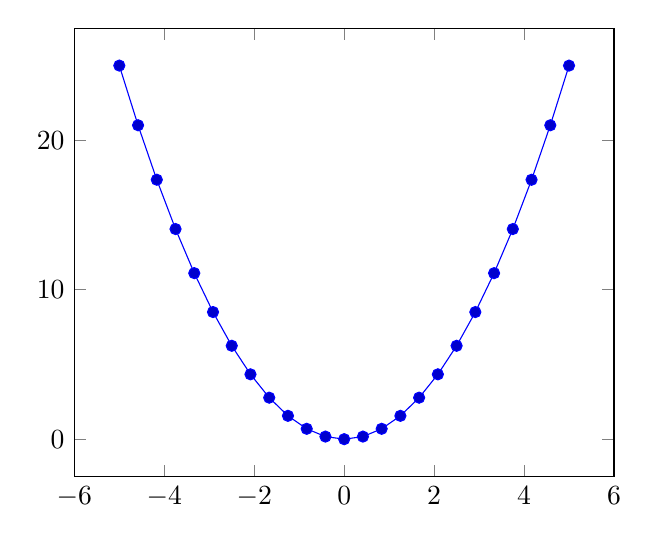
\begin{tikzpicture}
	\begin{axis}[]
	\addplot (\x,\x^2);
	\end{axis}
\end{tikzpicture}

\testsubsection{ymax=5}
\begin{tikzpicture}
	\begin{axis}[ymax=5]
	\addplot (\x,\x^2);
	\end{axis}
\end{tikzpicture}

\testsubsection{ymax=0.5}
\begin{tikzpicture}
	\begin{axis}[ymax=0.5]
	\addplot (\x,\x^2);
	\end{axis}
\end{tikzpicture}

\testsubsection{xmin=0}
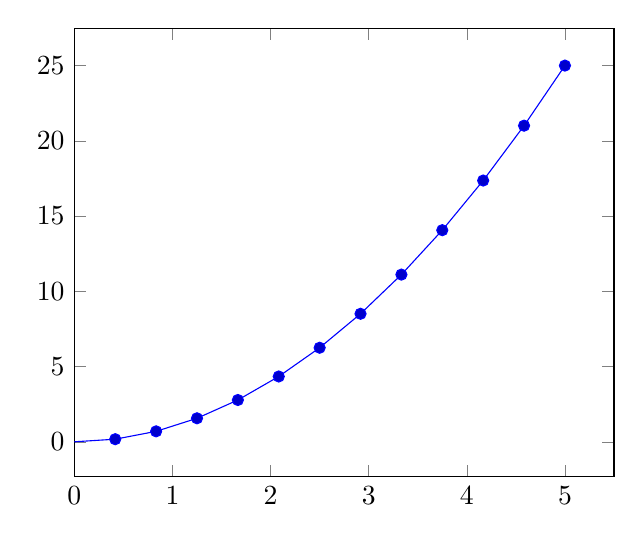
\begin{tikzpicture}
	\begin{axis}[xmin=0]
	\addplot (\x,\x^2);
	\end{axis}
\end{tikzpicture}

\testsubsection{xmin=768}
\begin{tikzpicture}
	\begin{loglogaxis}[xmin=768]
		\loglogtestplot
	\end{loglogaxis}
\end{tikzpicture}

\testsubsection{ymax=5.8e-4}
\begin{tikzpicture}
	\begin{loglogaxis}[ymax=5.8e-4]
		\loglogtestplot
	\end{loglogaxis}
\end{tikzpicture}

\testsubsection{constant in $y$}
\begin{tikzpicture}
	\begin{axis}
	\addplot coordinates {(0,500) (10,500)};
	\end{axis}
\end{tikzpicture}

\begin{tikzpicture}
	\begin{axis}
	\addplot coordinates {(0,51234500) (10,51234500)};
	\end{axis}
\end{tikzpicture}

\begin{tikzpicture}
	\begin{axis}
	\addplot coordinates {(10,0) (20,0)};
	\end{axis}
\end{tikzpicture}

\testsubsection{constant in $x$}
\begin{tikzpicture}
	\begin{axis}
	\addplot coordinates {(0,500) (0,600)};
	\end{axis}
\end{tikzpicture}

\begin{tikzpicture}
	\begin{axis}
	\addplot coordinates {(51234500,60) (51234500,90)};
	\end{axis}
\end{tikzpicture}
